\documentclass[11pt]{standalone}
\usepackage[usenames, dvipsnames]{color}
\usepackage[margin=1in,vmargin=1in]{geometry}
\usepackage[utf8]{inputenc}
\usepackage[english]{babel}
\usepackage{tikz}
\usepackage{pgfplots}
\usepackage{fancyhdr}
\pagestyle{fancy}
\usepackage{floatrow}
\usepackage[font=small,labelfont=bf,labelsep=period]{caption}
\usepackage{graphicx}
\usepackage{graphics}
\usepackage{amsmath}
\usepackage{amsthm}
\usepackage{amssymb}


\begin{document}
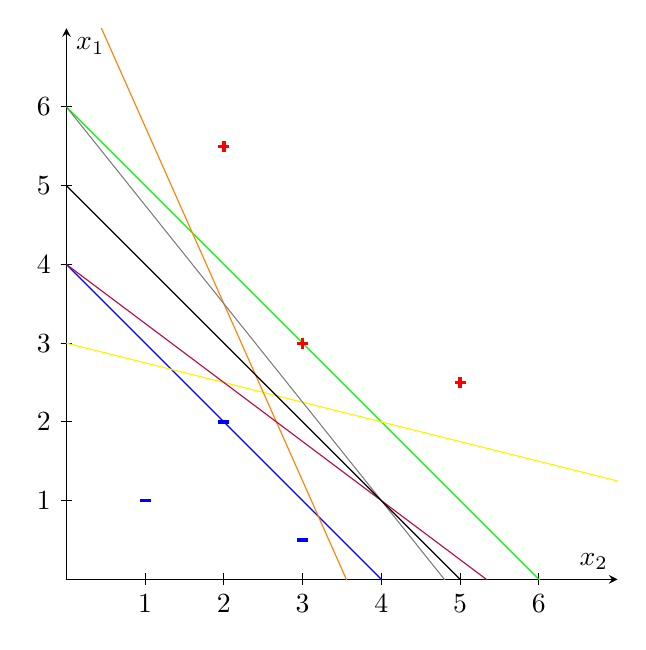
\begin{tikzpicture}[scale=1]
  \begin{axis}[x=1cm,y=1cm,
    axis x line=middle,
    axis y line=middle,
    ymin=0, ymax=7,
    ylabel=$x_{1}$,
    xmin=0, xmax=7,
    xlabel=$x_{2}$,
    ytick={1,2,3,4,5,6},
    xtick={1,2,3,4,5,6},
    xtick style={thin,black},
    ytick style={thin,black},]
    \addplot[blue,smooth,mark=none,domain=0:10]{-x+4};
    \addplot[green,smooth,mark=none,domain=0:10] {-x+6};
    \addplot[yellow,smooth,mark=none,domain=0:10] {-.25*x+3};
    \addplot[orange,smooth,mark=none,domain=0:10] {-2.25*x+8};
    \addplot[purple,smooth,mark=none,domain=0:10] {-.75*x+4};
    \addplot[gray,smooth,mark=none,domain=0:10] {-1.25*x+6};
    \addplot[black,smooth,mark=none,domain=0:10] {-x+5};
    \addplot[only marks,mark = +,red,very thick] coordinates{(3,3)(2,5.5)(5,2.5)};
    \addplot[only marks,mark = -,blue,very thick] coordinates{(2,2)(1,1)(3,.5)};
  \end{axis}
\end{tikzpicture}
\end{document}